\section{Escenarios}

\subsection{Crear Equipo}

En el siguiente escenario unParticipante crea un equipo eligiendo con el nombre Pipe\&Filter, el tecnico Popovich, el base LeBron James,escolta Kevin Durant, alero ShaquilleONeal, ala pivot Michael Jordan y como pivot Kobe Briant. 

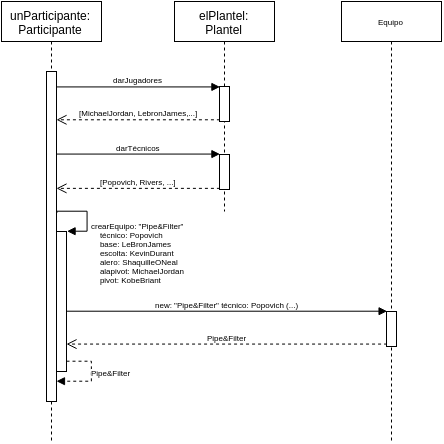
\includegraphics[width=\textwidth]{imgs/crearEquipoSecuencia.png}

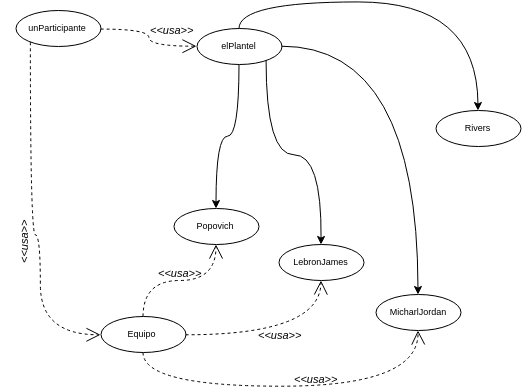
\includegraphics[width=\textwidth]{imgs/crearEquipoObjetos.png}



\subsection{Aceptar Desafío}
En este escenario otroParticipante elige de un pool de Desafíos el desafío donde está el equipo Pipe\&Filter apostando 5 fichas y lo acepta con su equipo llamado Batch. Luego el partido se simula y gana el equipo Pipe\&Filter 97 a 92 generando una ganancia de 15 fichas para unParticipante y una perdida de 5 fichas para otroParticipante. 

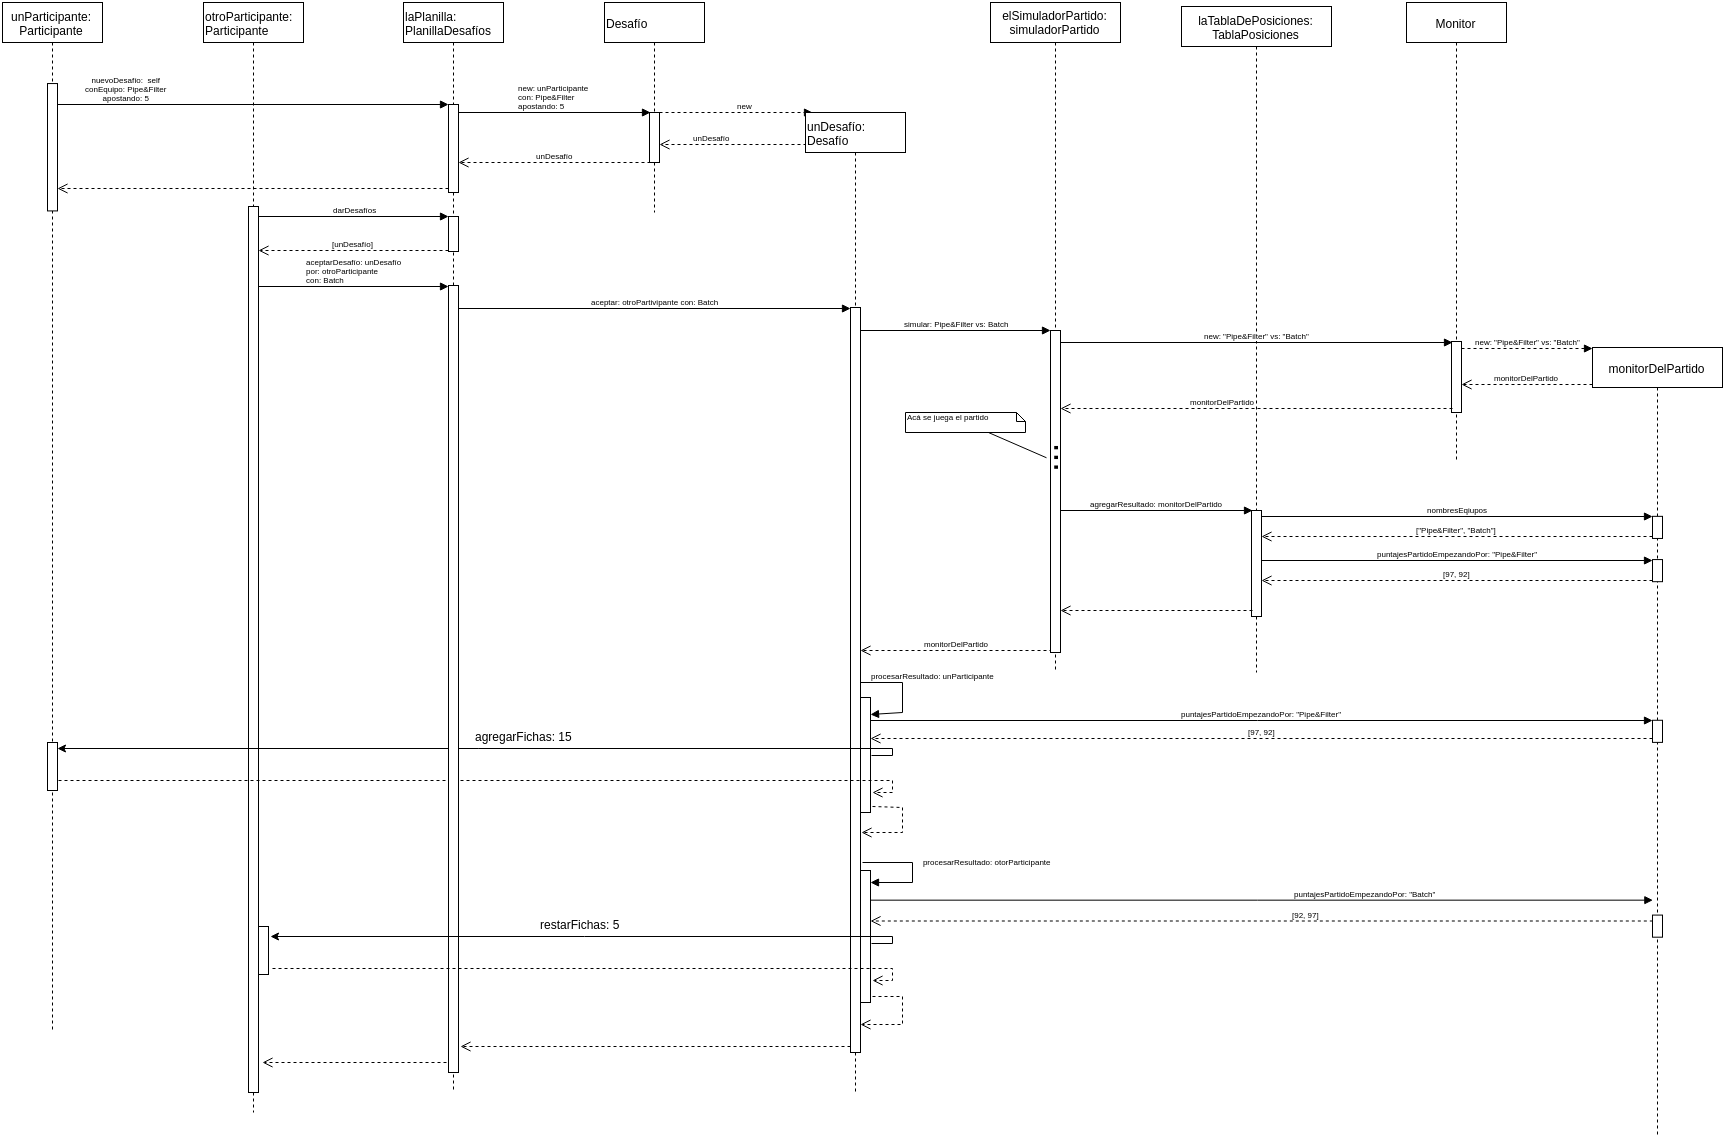
\includegraphics[height=0.7\textheight,keepaspectratio, angle =90 ]{imgs/aceptarDesafioSecuencia.png}

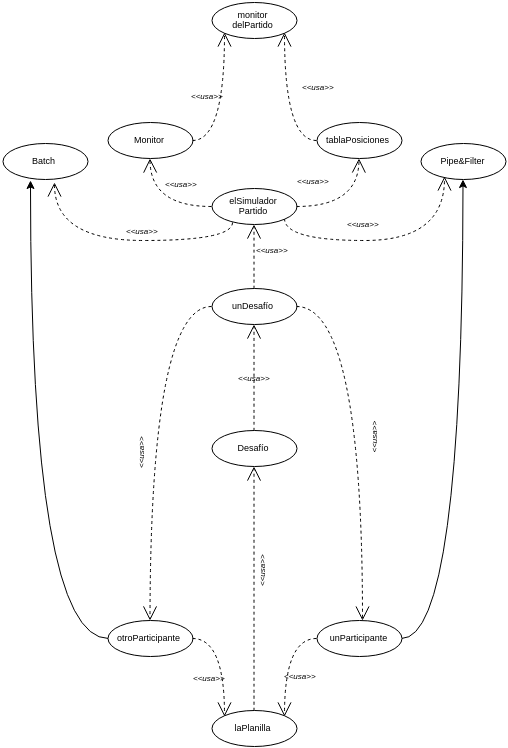
\includegraphics[width=\textwidth]{imgs/aceptarDesafioObjetos.png}

\subsection{Comiendo de un Partido}
Este diagrama muestra el "setup" inicial de la simulación de un partido, antes de que se comiencen a simular los turnos.

\includegraphics[width=\textwidth]{imgs/ComienzoDePartido.png}

\subsection{Pase Exitoso}

El siguiente diagrama muestra una secuencia de mensajes de un pase que es exitoso. Esta secuencia  se referenciará para simplificar los diagramas de las simulaciones del simuladorDeTurno.

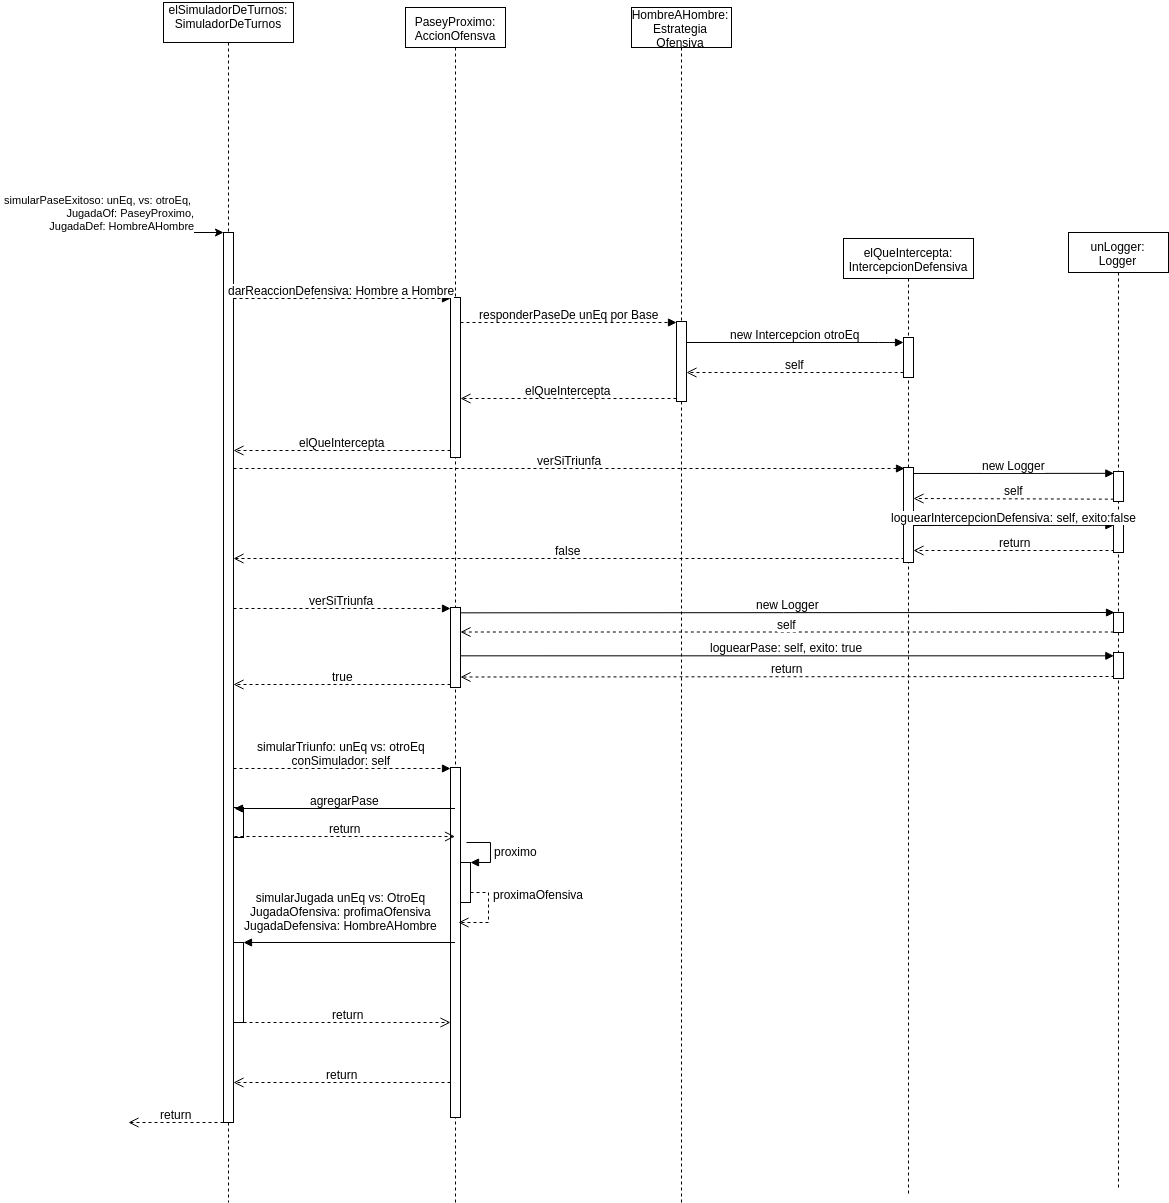
\includegraphics[width=\textwidth]{imgs/PaseExitoso.png}

\subsection{Pase Fallido}

Análogamente para el Pase Fallido

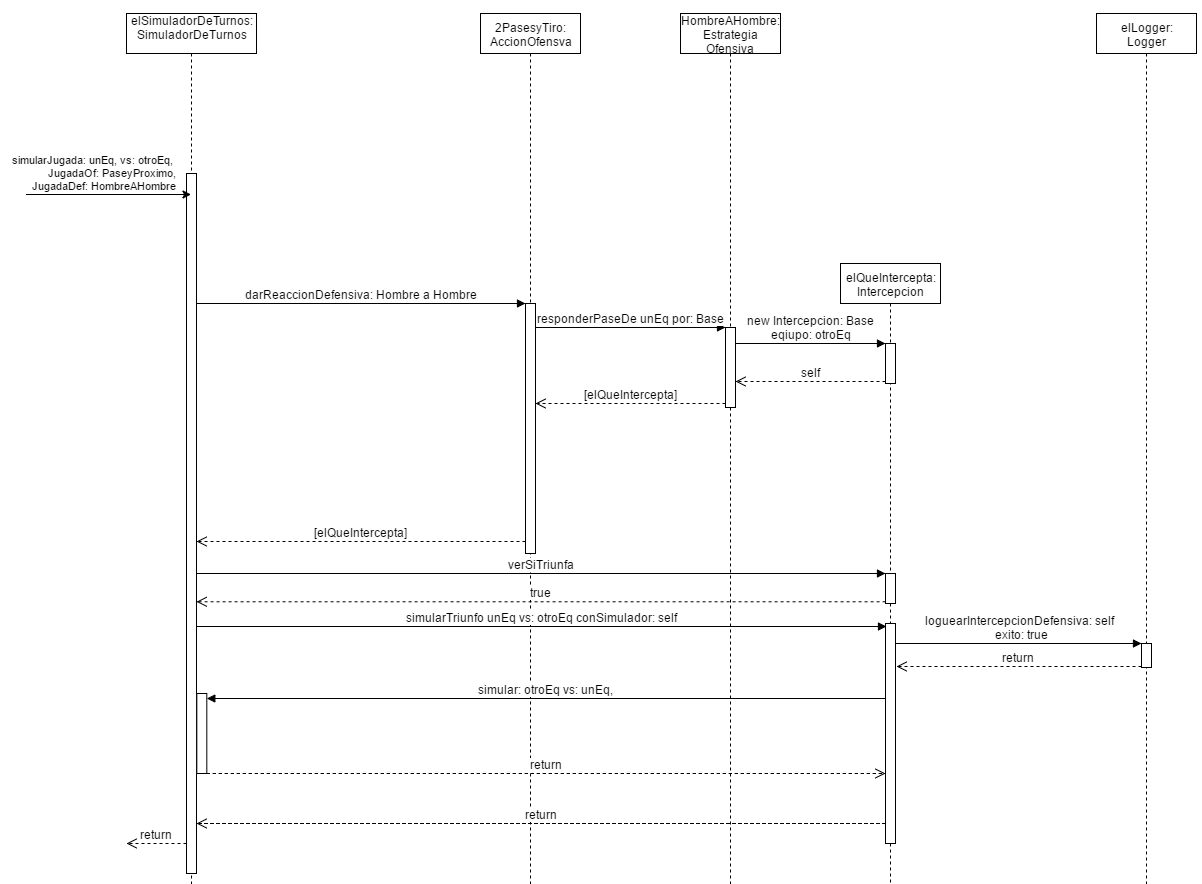
\includegraphics[width=\textwidth]{imgs/PaseFallido.png}

\subsection{Tiro Exitoso}

El siguiente diagrama muestra una secuencia de mensajes de un tiro que es exitoso. Esta secuencia se referenciará para simplificar los diagramas de las simulaciones del simuladorDeTurno.

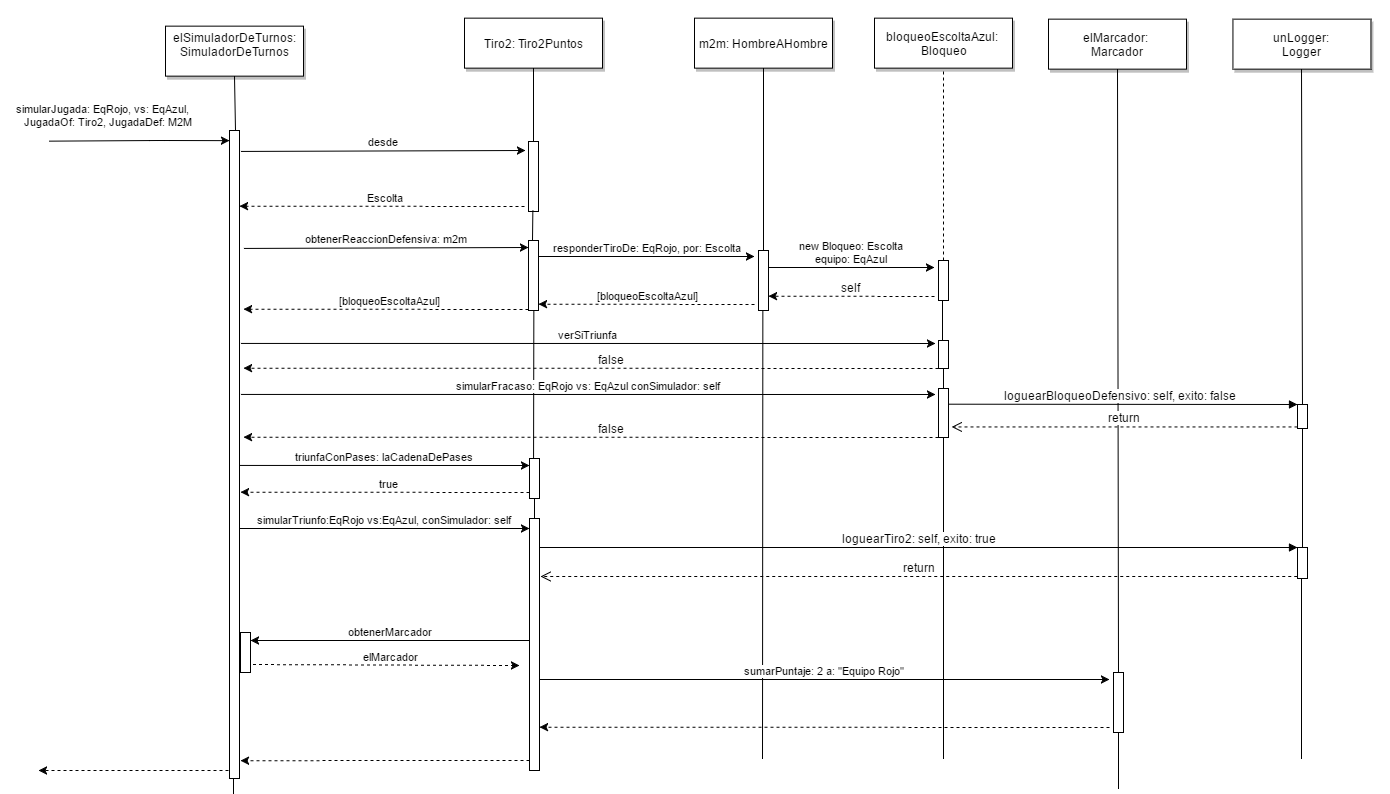
\includegraphics[height=0.60\textheight,keepaspectratio, angle =90 ]{imgs/TiroExitoso.png}

\subsection{Tiro Fallido}


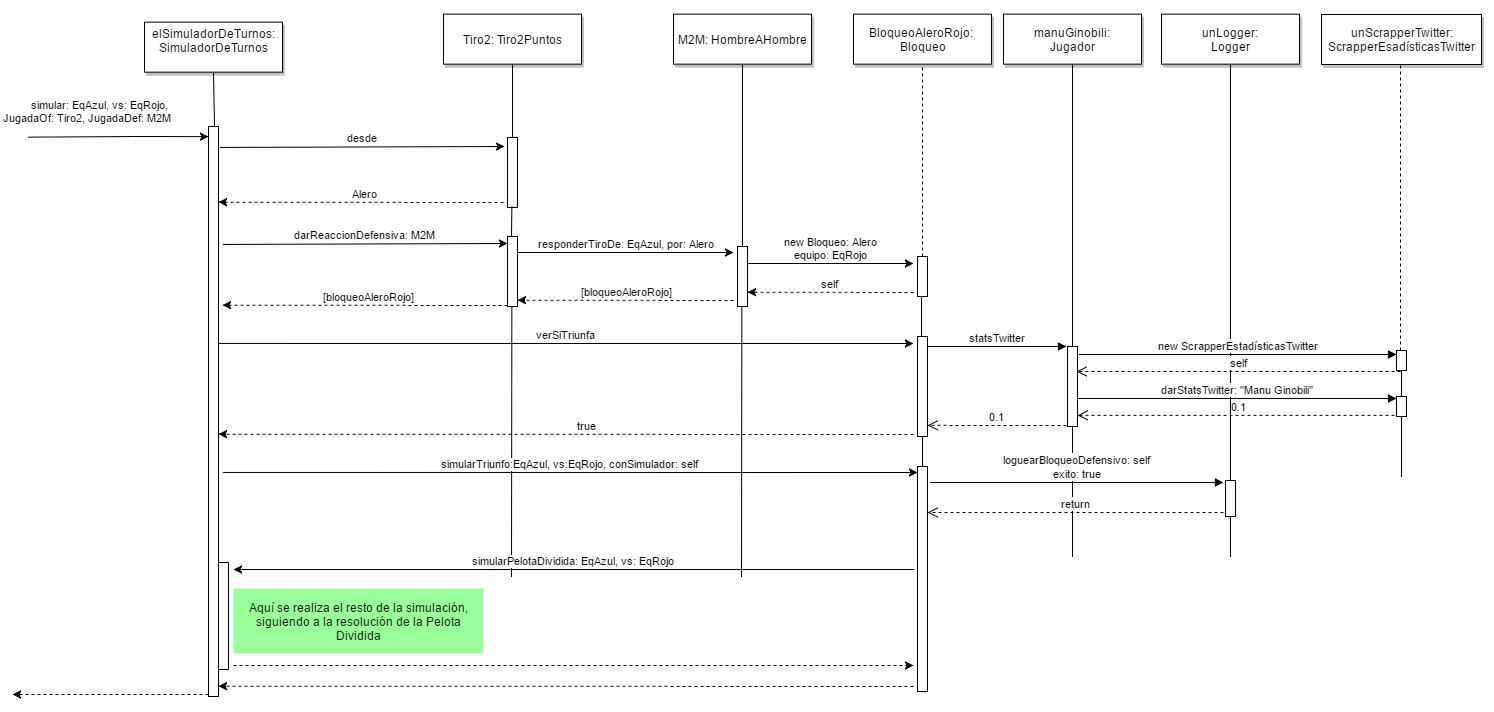
\includegraphics[height=0.45\textheight,keepaspectratio, angle =90 ]{imgs/TiroFallido.png}

\subsection{Pelota Dividida}

El siguiente diagrama muestra la resolución de una Pelota Dividida.

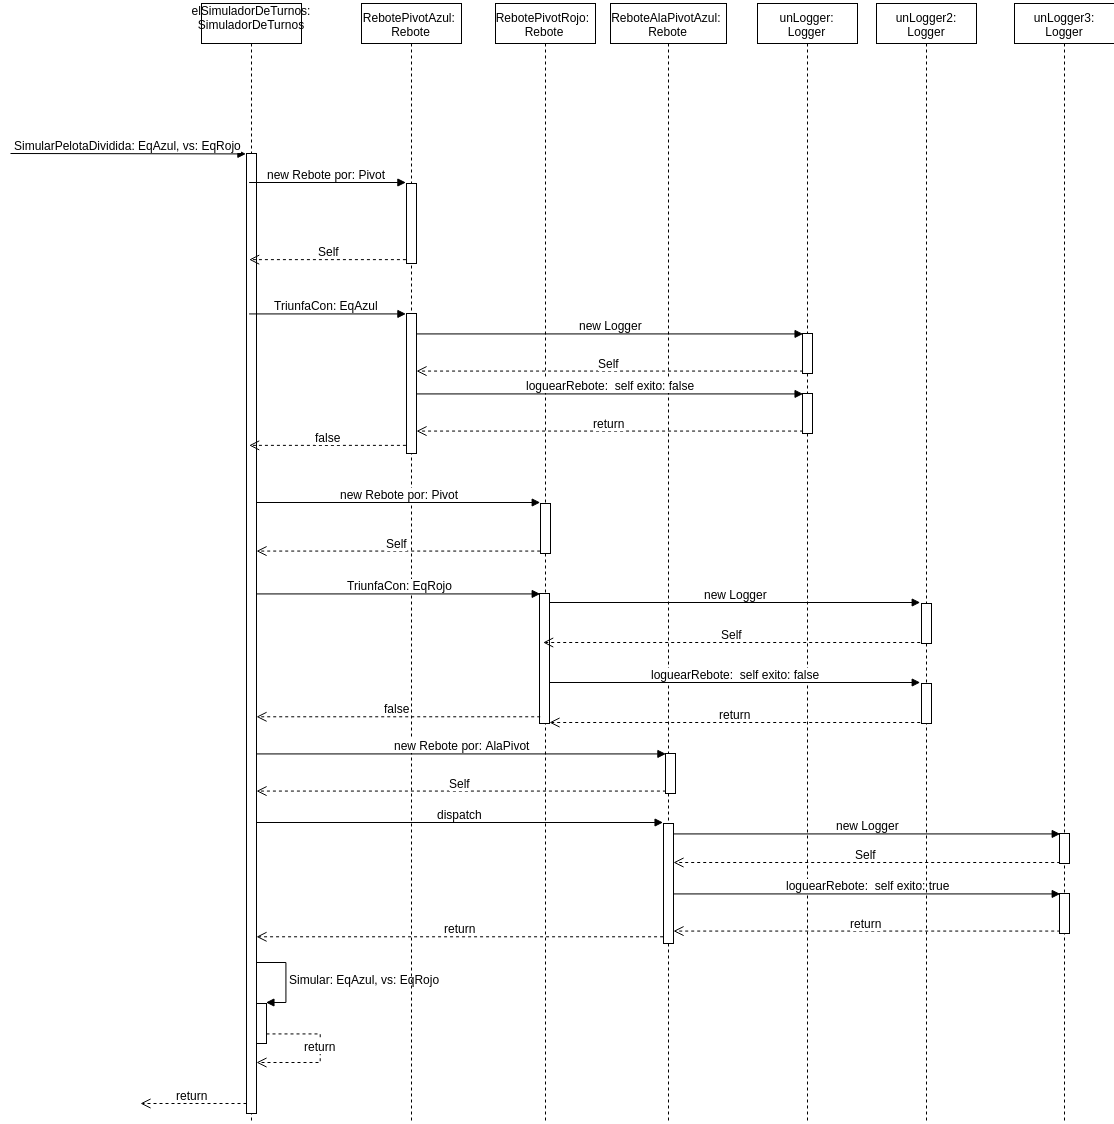
\includegraphics[width=\textwidth]{imgs/PelotaDivididaSecuencia.png}

\subsection{Colectiva Externa de 3}

El siguiente diagrama muestra un escenario donde en una jugada el equipo atacante (unEq) hace dos pases y un tiro y encesta, teneiendo como estrategia Colectiva Externa de k pases.

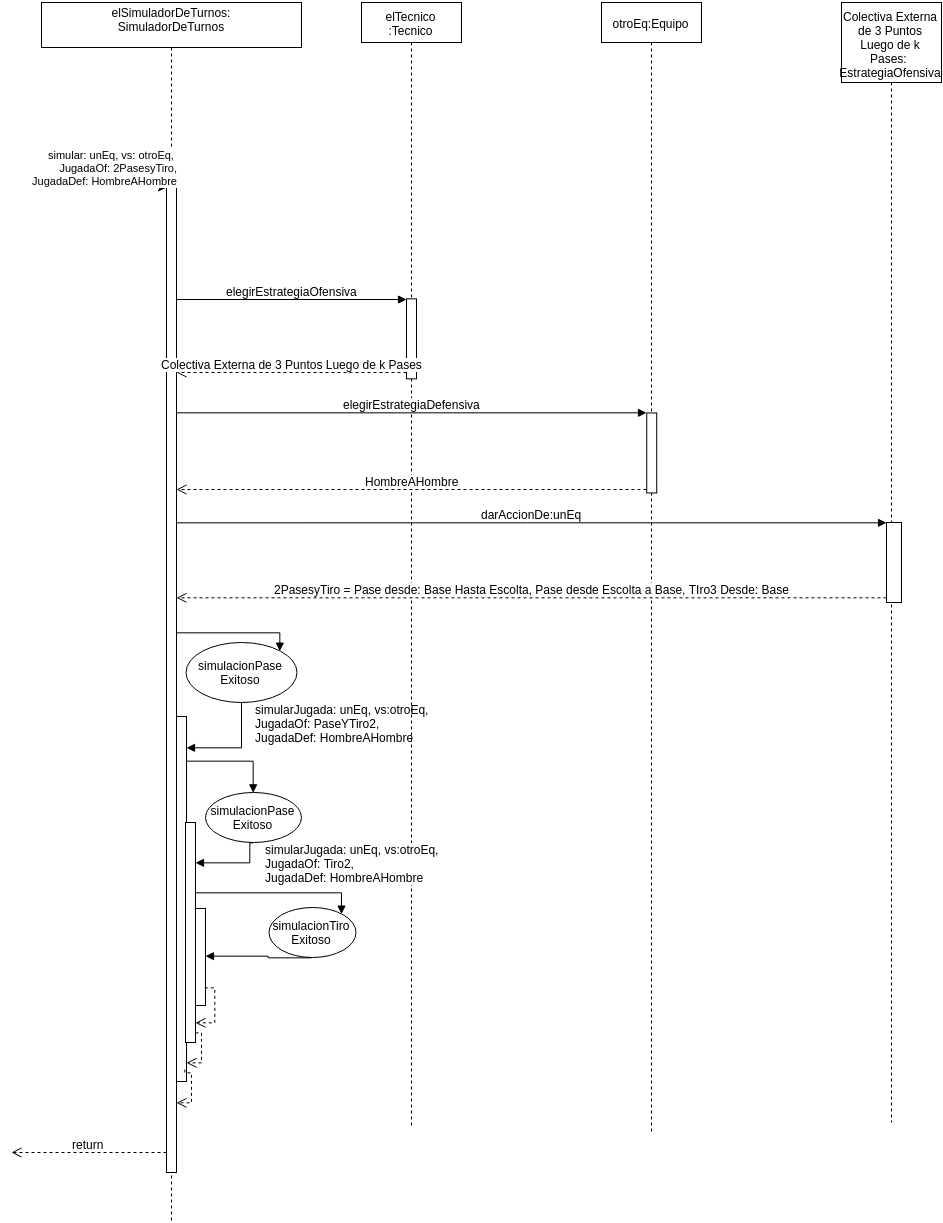
\includegraphics[width=\textwidth]{imgs/colectivaExternaDe3Secuencia.png}

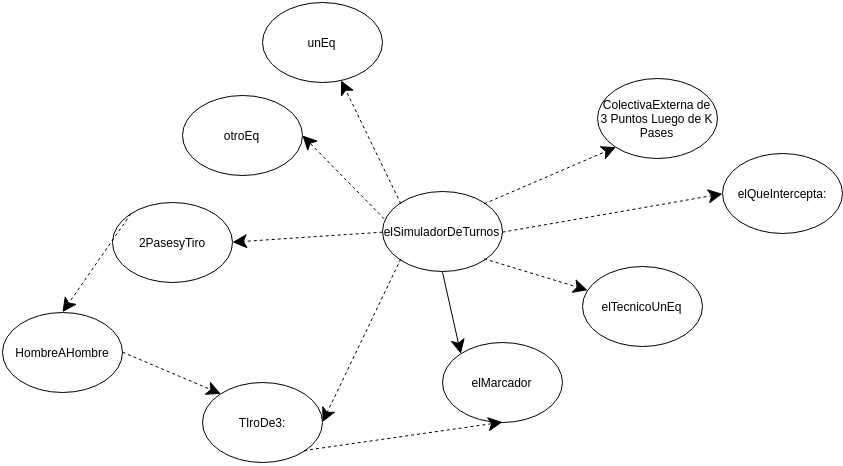
\includegraphics[width=\textwidth]{imgs/colectivaExternaDe3Objetos.png}

\subsection{Contraataque}

El siguiente diagrama muestra un escenario donde en una jugada el equipo atacante (eqAzul) hace un pase de forma exitosa (resumido como referencia al diagrama de Pase Exitoso), y en el segundo intento de pase es interceptado por el otro equipo y este ultimo contraataca tirando al aro y encestando, con lo cual suma 2 puntos al marcador para su equipo.

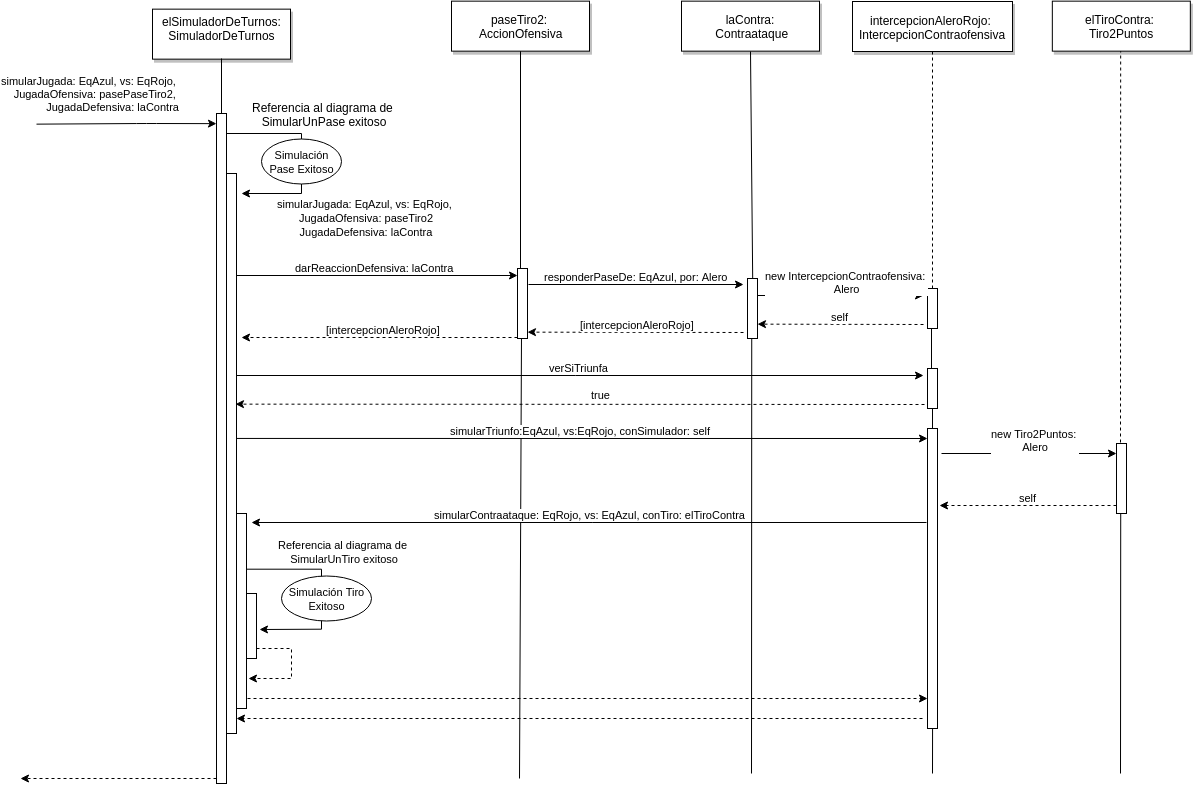
\includegraphics[width=\textwidth]{imgs/ContraataqueSecuencia.png}


